\documentclass[fleqn]{article}
\usepackage[utf8]{inputenc}
\usepackage[margin=2.5cm]{geometry}

% bibliography
\usepackage[round, sort&compress]{natbib}
\usepackage{har2nat}
\bibliographystyle{agsm}

% custom header/footer
\usepackage{fancyhdr}
\pagestyle{fancy}
\renewcommand{\headrulewidth}{0pt}
\fancyhf{}
\rfoot{\textsf{\thepage}}
\lfoot{\textsf{Suzie Brown}}

% miscellaneous formatting
\usepackage{xcolor}
\usepackage[font=small]{caption}
\usepackage{subcaption}
\usepackage{enumitem}

% tikz
\usepackage{tikz}
\usetikzlibrary{positioning}

% pseudocode
\usepackage{algorithm}
\usepackage{algorithmicx}
\usepackage{algpseudocode}

% maths
\usepackage{amsmath}
\usepackage{amssymb}
\usepackage{amsthm}
\newtheorem{lemma}{Lemma}
\newtheorem{remark}{Remark}
\newtheorem{corollary}{Corollary}
\newtheorem{conj}{Conjecture}
\theoremstyle{definition}
\newtheorem{defn}{Definition}

% useful math symbols
\newcommand{\PR}{\mathbb{P}}
\newcommand{\E}{\mathbb{E}}
\newcommand{\V}{\operatorname{Var}}
\newcommand{\eqdist}{\overset{d}{=}}
\newcommand{\I}[1]{\mathbb{I}_{\{#1\}}}
\newcommand{\Ntoinfty}{\overset{N\to\infty}{\longrightarrow}}
\newcommand{\limNtoinfty}{\underset{N\to\infty}{\lim}}
\newcommand\indep{\protect\mathpalette{\protect\independenT}{\perp}}
\def\independenT#1#2{\mathrel{\rlap{$#1#2$}\mkern2mu{#1#2}}}

% distributions
\newcommand{\Cat}{\operatorname{Categorical}}
\newcommand{\Unif}{\operatorname{Uniform}}
\newcommand{\Mn}{\operatorname{Multinomial}}
\newcommand{\Bin}{\operatorname{Binomial}}

% project-specific commands
\newcommand{\F}{\mathcal{F}_{t-1}}
\newcommand{\vt}[2][t]{\nu_{#1}^{(#2)}}
\newcommand{\wt}[2][t]{w_{#1}^{(#2)}}
\newcommand{\wbar}[2][t]{\bar{w}_{#1}^{(#2)}}
\newcommand{\vttilde}[2][t]{\tilde{v}_{#1}^{(#2)}}
\newcommand{\flnw}{\lfloor Nw_i \rfloor }

\title{Randomised roundings}
\author{Suzie Brown}
\date{\today}

\begin{document}
\maketitle
\thispagestyle{fancy}

\begin{defn}\label{defn:randround_1D}
Let $X\geq0$. A random variable $Y: \mathbb{R}_+ \to \mathbb{N}$ is a \emph{randomised rounding} of $X$ if $Y$ takes the values
\begin{equation*}
Y=
\begin{cases}
 \lfloor X \rfloor & \text{with probability } 1- X+ \lfloor X \rfloor \\
  \lfloor X \rfloor +1 & \text{with probability } X- \lfloor X \rfloor 
\end{cases}
\end{equation*}
\end{defn}
Note that we therefore have $\E[Y] =X$.

Definition \ref{defn:randround_1D} generalises easily to multivariate $X$. A randomised rounding of a vector $X \in \mathbb{R}_+^N$ produces a vector $Y \in \mathbb{N}^N$ such that $\E[Y]=X$. $Y$ can thus be used to construct an unbiased resampling scheme.

Such popular resampling schemes as systematic resampling and residual resampling with systematic residuals are based on randomised roundings. In each scheme, the marginal distributions of the offspring counts are as in Definition \ref{defn:randround_1D}, where $X=N\wt{i}$ and $Y=\vt{i}$. The variety in rounding-based schemes arises from the interactions between these individual offspring counts. 

In this document we will consider a general resampling scheme based on randomised rounding, and compare its genealogical properties to those of multinomial resampling.
Let $(w_1, \dots, w_N)$ be a normalised weight vector (that is, $w_i \geq 0$ and $\sum w_i = 1$), let $N\geq 2$ be an integer denoting the number of particles, and let $(v_1,\dots v_N)$ denote the resampled offspring numbers. We will attach a superscript $m$ or $r$ to denote offspring numbers corresponding to multinomial and rounding-based resampling respectively.

\begin{lemma}
For any $i \in \{1, \dots, N\}$,
\begin{equation*}
\E[(v_i)_2^{(m)} | w_i] \geq \E[(v_i)_2^{(r)} | w_i].
\end{equation*}
\end{lemma}

\begin{proof}
Using properties of the Multinomial distribution \citep{mosimann1962}, we have
\begin{equation*}
\E[(v_i)_2^{(m)} | w_i]  = N(N-1)w_i^2
\end{equation*}
Directly from Definition \ref{defn:randround_1D}, we calculate the corresponding quantity in the case of randomised rounding to be
\begin{align*}
\E[(v_i)_2^{(r)} | w_i] &= \flnw (\flnw -1) (1 - Nw_i + \flnw) + (\flnw +1) \flnw (Nw_i - \flnw) \\
&= \flnw \left( 2(Nw_i - \flnw) + \flnw -1 \right)
\end{align*}
We define the difference 
\begin{align*}
\Delta_i &:= \E[(v_i)_2^{(m)} | w_i] - \E[(v_i)_2^{(r)} | w_i] \\
&= N^2w_i^2 - Nw_i^2 - 2\flnw(Nw_i - \flnw) - \flnw^2 + \flnw \\
&= N^2 w_i^2 + \flnw^2 -2Nw_i \flnw - Nw_i^2 + \flnw \\
&= (Nw_i - \flnw)^2 - Nw_i^2 + \flnw 
\end{align*}
Then we have to show that $\Delta_i \geq 0$ for all $N\geq 2$ and $w_i \in [0,1]$. Consider the following cases.
\begin{description}
\item[Case] $w_i=k/N$ for some $k \in \{1, \dots, N-1\}$. \\
Then $\flnw = Nw_i = k$ and we have\\
$\Delta_i = 0 - k^2/N + k = k(1- k/N) \geq 0$.
\item[Case] $w_i \in (k/N, (k+1)/N )$ for some $k \in \{0, \dots, N-1\}$ \\
Then $\flnw = k$, and
\begin{align*}
\Delta_i &= (Nw_i - k)^2 - Nw_i^2 + k\\
&= N(N-1)w_i^2 - 2Nkw_i + k(k+1) \\
&= N(N-1) \left[ \left( w-\frac{k}{N-1} \right)^2 - \frac{k^2}{(N-1)^2} + \frac{k(k+1)}{N(N-1)} \right]\\
&= N(N-1) \left( w-\frac{k}{N-1} \right)^2 - \frac{k^2 N}{N-1} + k^2 +k \\
&\geq - \frac{k^2 N}{N-1} + k^2 +k \\
&= k\left(1-\frac{k}{N-1}\right)\\
&\geq 0
\end{align*}
\end{description}
For each $N$, any $w_i \in [0,1]$ falls into one of the above cases, so we conclude that $\Delta_i \geq 0$ for all $N, w_i$.
\end{proof}

\begin{figure}
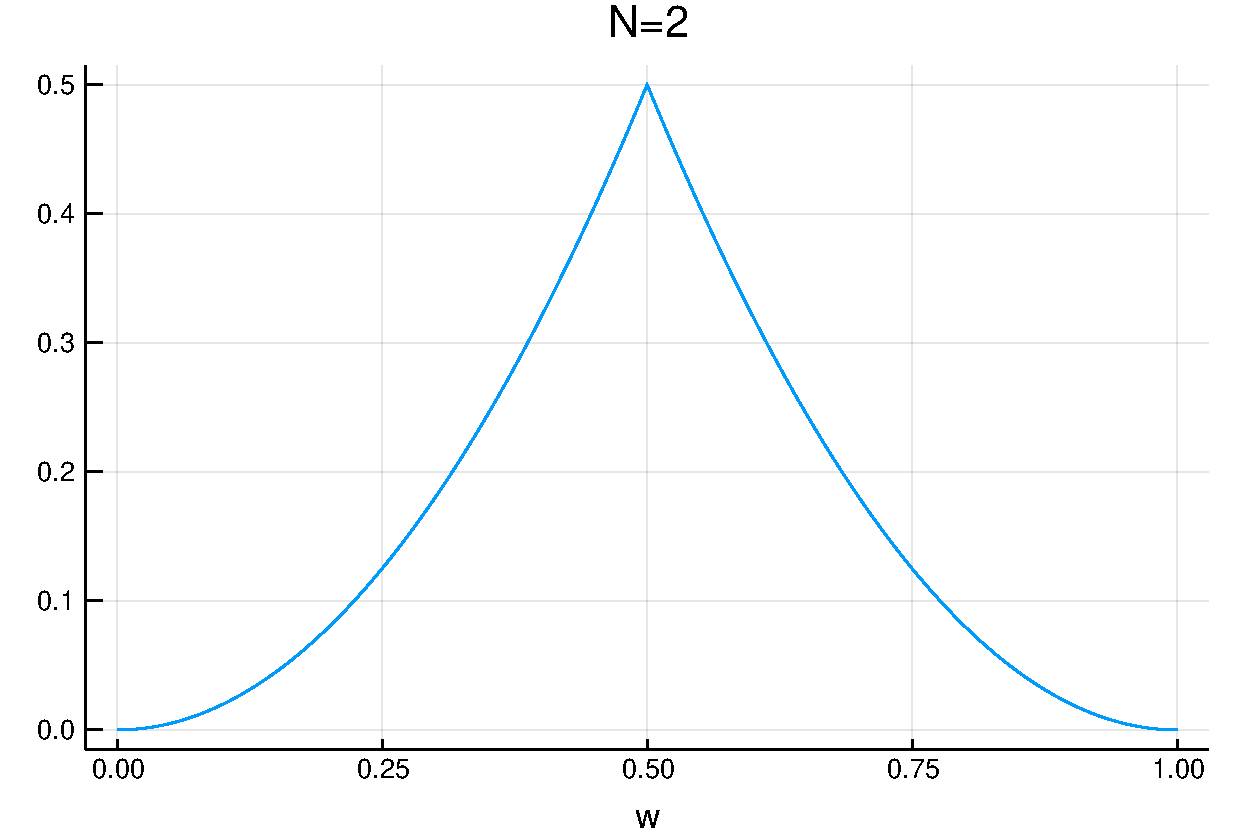
\includegraphics[width=0.33\textwidth]{plots/delta_cN_N2.pdf}
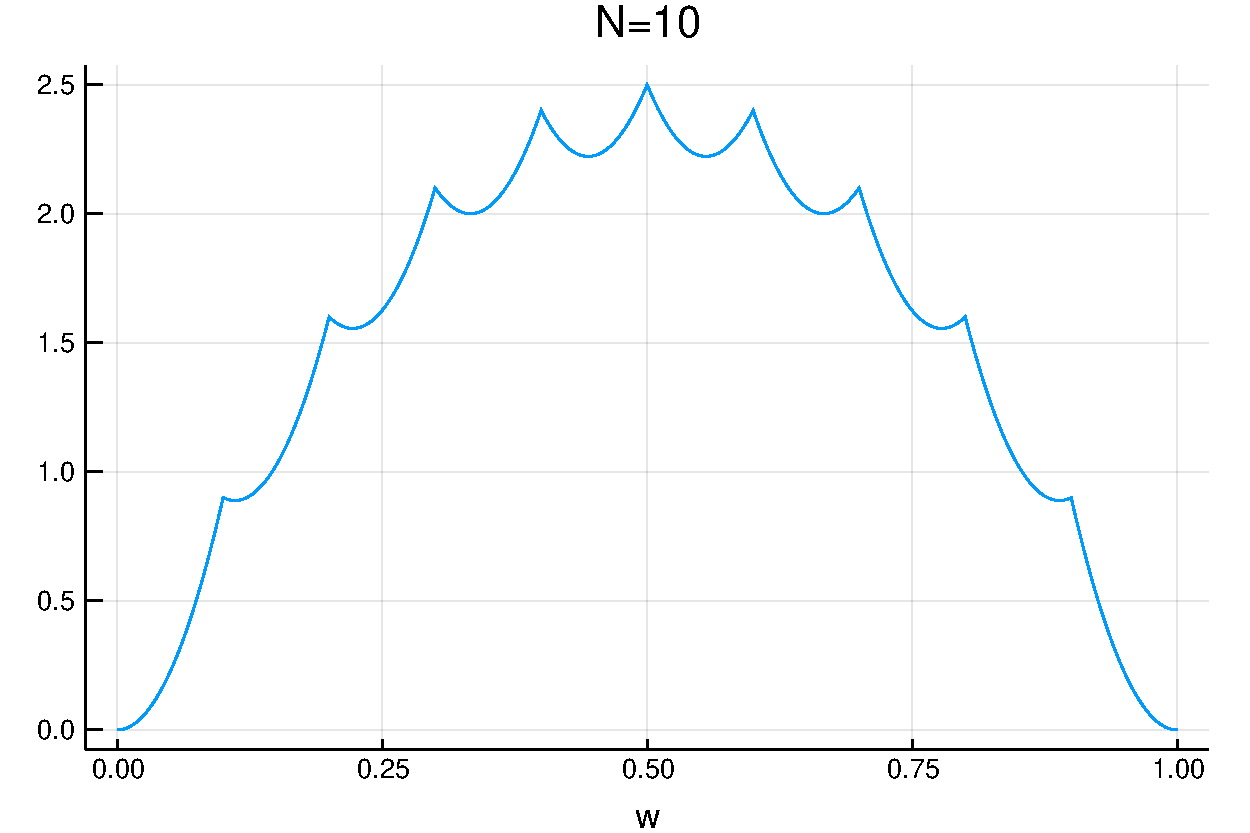
\includegraphics[width=0.33\textwidth]{plots/delta_cN_N10.pdf}
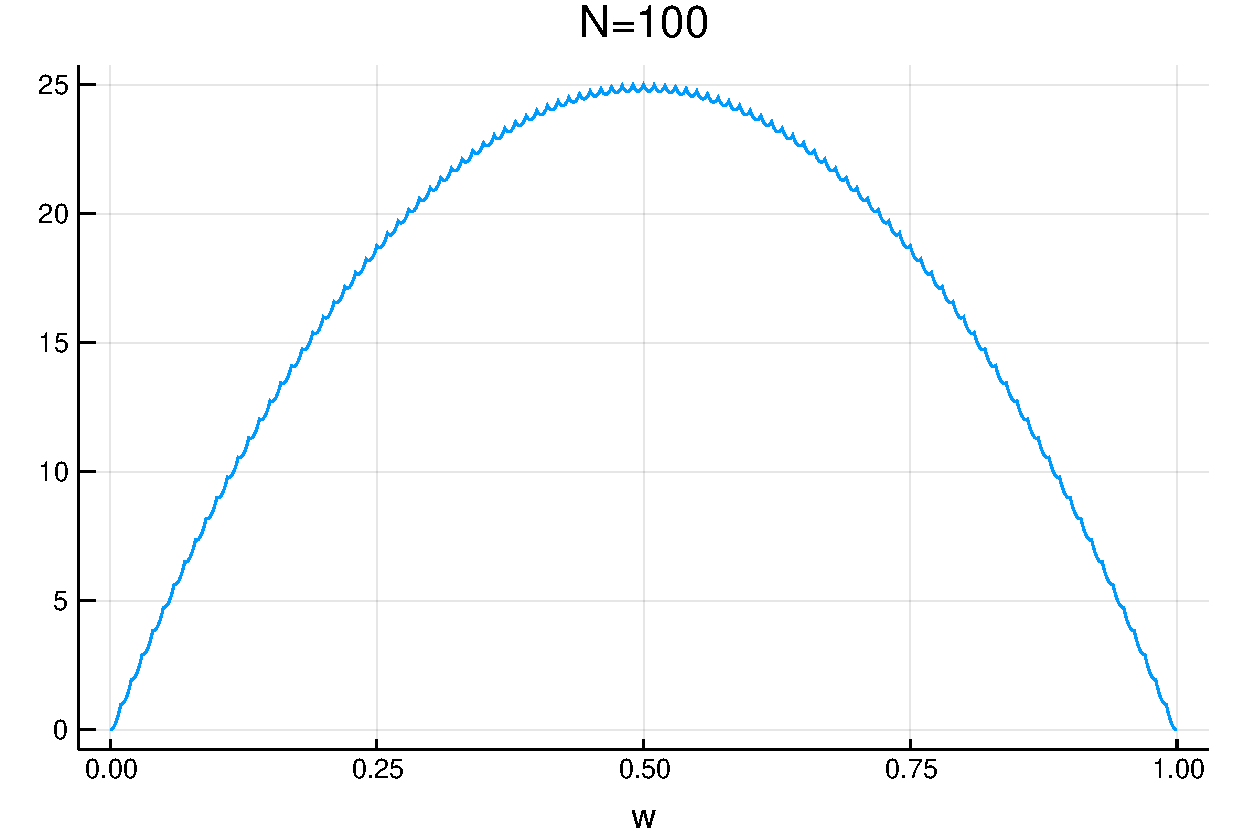
\includegraphics[width=0.33\textwidth]{plots/delta_cN_N100.pdf}
\caption{$\Delta_i$ as a function of $w_i$ for various values of $N$. The function is piecewise quadratic between the points $w_i = k/N$. The limiting shape appears to be a parabola.}
\end{figure}

\bibliography{../smc.bib}
\end{document}